\documentclass[a4paper,14pt]{article}
\usepackage{float}
\usepackage{extsizes}
\usepackage{amsmath}
\usepackage{amssymb}
\everymath{\displaystyle}
\usepackage{geometry}
\usepackage{fancyhdr}
\usepackage{multicol}
\usepackage{graphicx}
\usepackage[brazil]{babel}
\usepackage[shortlabels]{enumitem}
\usepackage{cancel}
\usepackage{textcomp}
\usepackage{array} % Para melhor formatação de tabelas
\usepackage{longtable}
\usepackage{booktabs}  % Para linhas horizontais mais bonitas
\usepackage{float}   % Para usar o modificador [H]
\usepackage{caption} % Para usar legendas em tabelas
\usepackage{tcolorbox}

\columnsep=2cm
\hoffset=0cm
\textwidth=8cm
\setlength{\columnseprule}{.1pt}
\setlength{\columnsep}{2cm}
\renewcommand{\headrulewidth}{0pt}
\geometry{top=1in, bottom=1in, left=0.7in, right=0.5in}

\pagestyle{fancy}
\fancyhf{}
\fancyfoot[C]{\thepage}

\begin{document}
	
	\noindent\textbf{6FMA94 - Matemática} 
	
	\begin{center}Revisão: formas descritivas (Versão estudante)
	\end{center}
	
	\noindent\textbf{Nome:} \underline{\hspace{10cm}}
	\noindent\textbf{Data:} \underline{\hspace{4cm}}
	
	%\section*{Questões de Matemática}
	~ \\ ~
	\begin{multicols}{2}
	\noindent Chamamos \textbf{forma descritiva} uma descrição ou uma forma descritiva com variáveis. \\
	Assim, por exemplo, são formas descritivas:
	\begin{itemize}
		\item 5
		\item $x$
		\item $a + x$
		\item $2x + 3y + 4z$
	\end{itemize}
	mas não são formas descritivas, por exemplo:
	\begin{itemize}
		\item 5 =
		\item 2 + 4 = 6
		\item $x + 5 = 7$
	\end{itemize}
	As duas últimas expressões linguísticas são chamadas \textbf{formas sentenciais}. \\
	No triângulo a seguir, uma descrição do seu perímetro é $a + b + c$.
	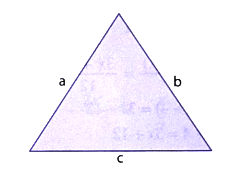
\includegraphics[width=1\linewidth]{imagens_6FMA94/imagem1}
	\end{multicols}
\noindent\textsubscript{~-----------------------------------------------------------------------------------------------------------------------------------------------------}
	\begin{multicols}{2}
    	\begin{enumerate}
    		\item Dado o retângulo a seguir: \\
    		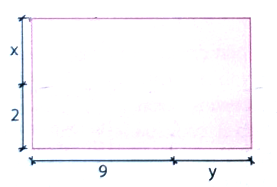
\includegraphics[width=1\linewidth]{imagens_6FMA94/imagem2}
    		\begin{enumerate}[a)]
    			\item apresentar uma descrição do seu perímetro. \\\\
    			\item apresentar uma descrição da sua área. \\\\\\\\\\
    		\end{enumerate}
    		\item O produto de dois números é 15. Se um dos números é x, escreva uma forma descritiva do outro número. \\\\
    		\item Rogério tem 26 anos e dois irmãos: Luciano, de $x$ anos, e Maurício. A idade de Maurício é a média das idades de seus irmãos. Obtenha uma forma descritiva com variáveis para indicar a idade dele. \\\\\\\\\\
    		\item Complete o enunciado seguinte com algum número do quadro abaixo e, em seguida, resolva o problema:
    		
    		\noindent \begin{tcolorbox}[colback=white, colframe=black, boxrule=0.5mm, width=8cm]
    			182 ~ 174 ~ 193 ~ 185 ~ 179 ~ 191
    		\end{tcolorbox}
    		Em um time de vôlei, duas jogadoras, Ana e Bianca, têm \underline{~~~~~~~~~} cm e $y$ cm de altura, respectivamente. Sabendo que a altura da jogadora Clara é igual à média das alturas de Ana e Bianca, obtenha uma forma descritiva com variáveis para indicar a altura de Clara em cm. \\\\\\\\\\\\\\\\\\\\\\\\
    		\item Em uma concessionária há $x$ carros pretos e $y$ carros vermelhos. Ao fazer o levantamento da loja, um vendedor notou que o número de motos era o quádruplo do número de carros. Escreva uma forma descritiva com variáveis para representar o número de:
    		\begin{enumerate}[a)]
    			\item carros na concessionária. \\\\\\\\\\
    			\item motos na concessionária. \\\\\\\\\\
    		\end{enumerate}
    		\item Dado o retângulo a seguir:
    		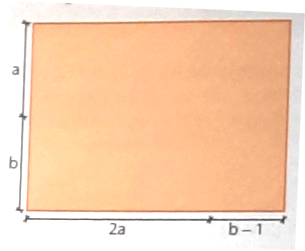
\includegraphics[width=1\linewidth]{imagens_6FMA94/imagem3}
    		\begin{enumerate}[a)]
    			\item apresentar uma descrição do seu perímetro. \\\\\\\\\\
    			\item apresentar uma descrição da sua área. \\\\
    		\end{enumerate}
    		\item A soma de três números é 80. Um dos números é $x$ e o segundo é o triplo de $x$ menos 5 unidades. Escreva uma forma descritiva do terceiro número. \\\\\\\\\\\\\\
    		\item O quociente de dois números não nulos é 7. Se o divisor é $x$, como podemos descrever o dividendo? \\\\\\\\\\\\\\
    		\item Joana têm três primos. Um deles tem 164 cm de altura e os outros dois têm $x$ cm e $y$ cm. A altura de Joana é a média das alturas dos seus primos. Obtenha uma forma descritiva com variáveis para descrever a altura dela. \\\\\\\\\\\\\\\\\\\\
    		\item Complete o seguinte enunciado com algum número do quadro abaixo e, em seguida, resolva o problema.
    		\noindent
    		\begin{center} \begin{tcolorbox}[colback=white, colframe=black, boxrule=0.5mm, width=6cm]
    			7 ~ 9 ~ 14 ~ 8 ~ 12 ~ 5
    		\end{tcolorbox}
    		\end{center}
    		Marcelo e seus primos notaram uma relação entre suas idades: a idade de Eduardo somada ao triplo da idade de Igor é igual ao dobro da idade de Marcelo. Sabendo que Eduardo tem ...... anos e Igor $x$ anos, obtenha uma forma descritiva com variáveis para descrever a idade de Marcelo.
    	\end{enumerate}
    $~$ \\ $~$ \\ $~$ \\ $~$ \\ $~$ \\ $~$ \\ $~$ \\ $~$ \\ $~$ \\ $~$  \\ $~$  \\ $~$  \\ $~$  \\ $~$  \\ $~$  \\ $~$  \\ $~$  \\ $~$ \\ $~$
	\end{multicols}
\end{document}